\articlehead{Makyo's Kaddish}{Makyo}{2012}

The about page mentions as much but I'll restate it more in-depth here.  I wound up at Colorado State University for college, starting in biochemistry but quickly moving to music.  I wound up spending longer than usual in the program for a few reasons.  First of all, I started off in music education.  That lasted for a few years, until I got far enough in the degree to start taking education classes, which didn't sit well for me.  They were all about obeying the law and not getting sued by parents, rather than teaching children effectively.  After that, I switched to music composition.

Unfortunately, there wasn't really a music composition program at my school, since there wasn't really a music composition professor.  There was an adjunct professor that taught orchestration, improvisation, and jazz theory classes, though, and he wound up being my main professor for about a year.  However, I wasn't the only one switching into the program at the time, so the university began the search for a composition chair.  I was lucky enough to be in on the selection process and helped to pick CSU's current composition professor, and we wound up with a wonderful guy to head the department.  One of the first things he nudged me towards after listening to some of my composition assignments was Leonard Bernstein's symphonies, and the one I fell in love with immediately was the third, Kaddish.

Kaddish, specifically the Mourner's Kaddish, is a Jewish prayer singing the praises of God.  In his symphony, Bernstein mingles the text of the Kaddish, sung in the choir, with a narration that I feel describes an important transition that many people go through, both individually and as societies and cultures.

The piece opens with an introduction from the narrator describing God as ``lonely, disappointed father'' and ``angry, wrinkled old majesty''.  The tone is immediately set, and not simply by the words.  The first sounds the listener hears are actually the entire choir humming an indeterminate pitch sotto voce. The effect is close to a science fiction movie's depiction of space, but gives the impression of a vast and frightening expanse.  As the piece progresses and the choir starts to sing the words of the Kaddish, chaos breaks out with loud percussion and bright brass.  This isn't a happy song singing the virtues of the Lord.

On the return of the narrator, one hears why: ``you [\ldots] who cause the dawn to know its place, surely you can cause and command a touch of order here below on this one dazed speck.''  The narrator isn't pleased about his relationship with his God (who never replies in the piece, except perhaps through music).  As the piece continues, the confrontation between the narrator and God escalating to a climax as the narrator accuses God of breaking his covenant to man after the flooding of the earth.  ``Tin God,'' he screams, ``Your bargain is tin!  It crumples in my hand!  And where is faith now, Yours or mine?!''

As the symphony winds on, the narrator compares and contrasts the idyllic world of God's creation of the Kingdom of Heaven with the reality that man has created, all in the guise of a dream.  The Kingdom of Heaven is ``just as You planned it, every immortal cliché intact'' where as the world of man is filled with ``Real-life marvels! Genuine wonders! Dazzling miracles!''  As the narrator and God awaken, the narrator proposes a new covenant, ``not quite the covenant we bargained for so long ago,'' and pledges that the two shall always ``Suffer and recreate each other.''  On this new agreement, the piece comes to a crashing end.

I know I need to tie this back to my own experiences with furry, but it requires a bit of explanation first.  First, I have to admit that if I'm unschooled in the ways of sociology and anthropology, I'm even more ignorant in theology and apologetics.  From the little I've read, though I've come to understand that the relationship between the both Christians and Jews and God is not a static thing, beyond the base definition of Creator and Created.  The relationship changed when Abraham obeyed God's command to sacrifice Isaac; it changed after the biblical flood with the aforementioned covenant; it changed with Moses, with David, and with Jesus.  It's still changing.

\begin{wrapfigure}{l}{0.3\textwidth}
  \begin{center}
    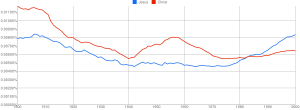
\includegraphics[width=0.25\textwidth]{content/assets/makyos-kaddish--j-v-c}
  \end{center}
  \caption{`Jesus' vs. `Christ'}
\end{wrapfigure}

The chart to the side displays uses of the terms ``Jesus'' and ``Christ'' between the years 1900 and 2000.  During the late '80s and into the '90s, you can see how the trend shifts away from ``Christ'' and toward ``Jesus''.  I believe, and this is only a gut-reaction, that this is largely due to the more personal relationship with one's God being preached in the last few decades with the growth of large evangelical and liberal Christian churches.  Clearly, the change is still coming within something as established as western religion.

So what does this have to do with furry?.  There's been a lot of my own path through the fandom that matches up closely with the narrator's growth in his relationship with God.  Most importantly, the similarities are evident when, at the end of Bernstein's Kaddish, the narrator and God come to a new covenant wherein they suffer and recreate each other.

This is something I spend a lot of time thinking about.  I've been chugging along in the fandom for about twelve years now.  I was initially pretty happy to just go along with whatever everyone else was doing, and even after I stopped doing that, I was still pretty happy to just say I was a part of it.  I was a furry and pretty cool with it.  I couldn't draw, didn't have much money to buy commissions, didn't have a fursuit, and talked almost exclusively with my own little group of friends.  Then I got bitter.

Around my second or third year of college, after I'd been going to the local meets for a while, I found that, more often than not, I wasn't really happy with the fandom.  It's not that I didn't like where it was going, so much that I didn't like that I was in it.  I was occasionally ashamed by the fact that I was a fur, and that made me feel sort of sarcastic about the whole thing.  Of course, that worked pretty well as a feedback loop, and I started to sort of wind down my life within the fandom.  I talked to fewer and fewer people, I went to less and less meets.  I still went to cons, but I stopped going to panels.  I started making money, but never really used it to buy commissions.  I wound up changing my name to distance myself from the past -- whereas before I was Ranna, the red fox who stole a cool sounding name from a book, now I was Makyo, the arctic fox whose name meant a demon that distracts from the path to enlightenment (I thought it was witty for a future teacher).

It wasn't necessarily that I wanted to get out of the fandom.  With the few friends I still interacted closely with, including one wonderful partner, I was still a fox guy.  I still kept up on enough of the goings on to have intelligent conversations with the people I did talk to.  Even so, I felt like I was going to what I thought was the standard thing: stick around furry for five to ten years, then leave it once real life took over.  It stung, at first, but I figured I was growing up.

Eventually, the snarky attitude calmed down and I settled into a routine with those around me.  It took me accidentally embedding myself in a portion of the Colorado furs, a chance invitation to a party, a few more people showing up at the local meets, and moving to an apartment building that hosted other furs.  It was the deeper sense of meaningful communication that I got from my furry friends that seemed to be missing from my music friends that got me thinking that I needed to renegotiate my membership within the fandom.  I wasn't content to just be a listless member anymore, I wanted to be an active participant.

This was, of course, still a few years ago.  At the time, I began by trying to post more to my FA account.  I posted my music, which garnered little to no attention.  I commissioned some more art, which got a little more.  That attention felt good.  It was good to be known, to some (very) small extent by the art that I commissioned.  I can understand individuals who get a lot of art of their characters done, now: it just feels good.  It's the visible affirmation of our character, and the affirmation of our social worth when the work is appreciated.

Even so, I wanted more.  I wanted to be on more even ground with the subculture of which I was a part.  I don't think I'm the only one to experience this, either.  Sites such as The Furry Agenda, SoFurry, and so many others all aim to give back the fandom, yet are the products of their creators.  The same could be said vis-à-vis conventions and their chairs and board-members.  For me, the next part happened by accident.

My rather furry boss (hey boss, promise I'm writing this at home!) and I were joking around one day just after Halloween.  On the holiday, there was a party -- small convention, even -- and a friend of mine mentioned that there sure were a lot of people who were named ColorSpecies or some variant.  I don't know who it was that my friend had talked to, but I brought it up to my boss and we wound up coming up with an idea to make some goofy automatic textual description generator that would fill in a template a-la the roadtrip game Ad-Libs.

I registered adjectivespecies.com that afternoon.

I'm not really sure how I got from the idea of ad-libbing descriptions to this loose amalgam of meta-furriness that we have now.  It happened quickly, of course.  I registered the domain that afternoon, and wrote the first article that night.  It probably had much to do with the drive home (my commute is about an hour long).  During the drive, I think I realized that what I was originally planning was much closer to my more sarcastic days than what I was aiming for.  I didn't want to just wind up as some snarky, burned fur blogger making a snarky, burned fur website.

What was I aiming for?  I'm still not sure.  The recognition, a little bit; I did want to make a bit of a name for myself within the fandom, but it wasn't just that (there certainly are easier ways about it, too).  To create a resource of introspection, too; I think that introspection is an important tool for anyone, especially when it comes to intangibles, and many of my previous projects reflected that.  More than anything, though, I wanted to, like the narrator and God within Kaddish, work with the fandom, dream with it, understand it.  Nothing so grandiose as changing furry to fit my whims, of course, it's not my place to do so; simply to explore and grow along with it.  This was my new covenant with myself as an individual and myself as a member of the subculture: that we should continuously suffer and recreate each other.
